\section{Validation on Simulated Data} %Toy Example
\label{sec:experiment_toy}
%\vspace{-3mm}

%

%    	A scenario with random identity switches renders relational reasoning necessary for accurate prediction of location in next time step. Circles of the same colour repel each other, circles of different colours attract each other. The colour coded identities are randomly assigned in each time step rendering information exchange between trackers (i.e. relational reasoning) necessary. While \textsc{hart} (top, $46\%$ IoU) clearly struggles in this stochastic environment, \textsc{mohart} (bottom, $76\%$ IoU) predicts the future locations much more accurately. The numbers in the bottom row indicate the self-attention weights from the perspective of the top left tracker (yellow number box).
%    	\textsc{hart} (top, $46\%$ IoU) vs. \textsc{mohart} (bottom, $76\%$ IoU). Dashed lines show spatial attention, solid lines show predicted bounding boxes, faded circles indicate future ground truth locations. Circles of the same colour repel each other, circles of different colours attract each other. The colour coded identities are randomly assigned in each time step rendering information exchange between trackers (i.e. relational reasoning) necessary. The numbers in the bottom row indicate the self-attention weights from the perspective of the top left tracker (yellow number box).

We test and compare the relational reasoning capabilities of the proposed algorithms on a toy domain. The domain is a 2D squared box which contains circular objects with approximated elastic collisions (energy and momentum conservation) between objects and with walls. To investigate how the model understands motion patterns and interactions between objects, we train it to predict future object locations in contrast to traditional tracking.

In the first experiment, each circle exerts repulsive forces on each other, where the force scales with $1/r$, $r$ being the distance between them. Predicting the future location just using the previous motion of one object (i.e. without relational reasoning) accurately is therefore challenging. We show that \textsc{hart} as an end-to-end single-object tracker is able to capture complex motion patterns and leverage these to make accurate predictions (see \Cref{sec:appendix_toy}). This indicates that \textsc{hart} is able to draw conclusions about the (deterministic, but not static) force field.

%In the first scenario (\Cref{fig:toy1}), four circles each exert repulsive forces on each other, where the force scales with $1/r$, $r$ being their distance. \textsc{hart} is applied four times in parallel and is trained to predict the location of each circle three time steps into the future. The different forces from different objects lead to a non-trivial force field at each time step. Predicting the future location just using the previous motion of one object (\Cref{fig:toy1} shows that each spatial attention box covers only the current object) accurately is therefore challenging. Surprisingly, the single object tracker solves this task with an average of $95\%$ IoU over sequences of 15 time steps. This shows the efficacy of end-to-end tracking to capture complex motion patterns and use them to predict future locations. This, of course, could also be used to generate robust bounding boxes for a tracking task.

\begin{figure}
    \centering
    \begin{subfigure}[c]{0.49\linewidth}
        \centering
        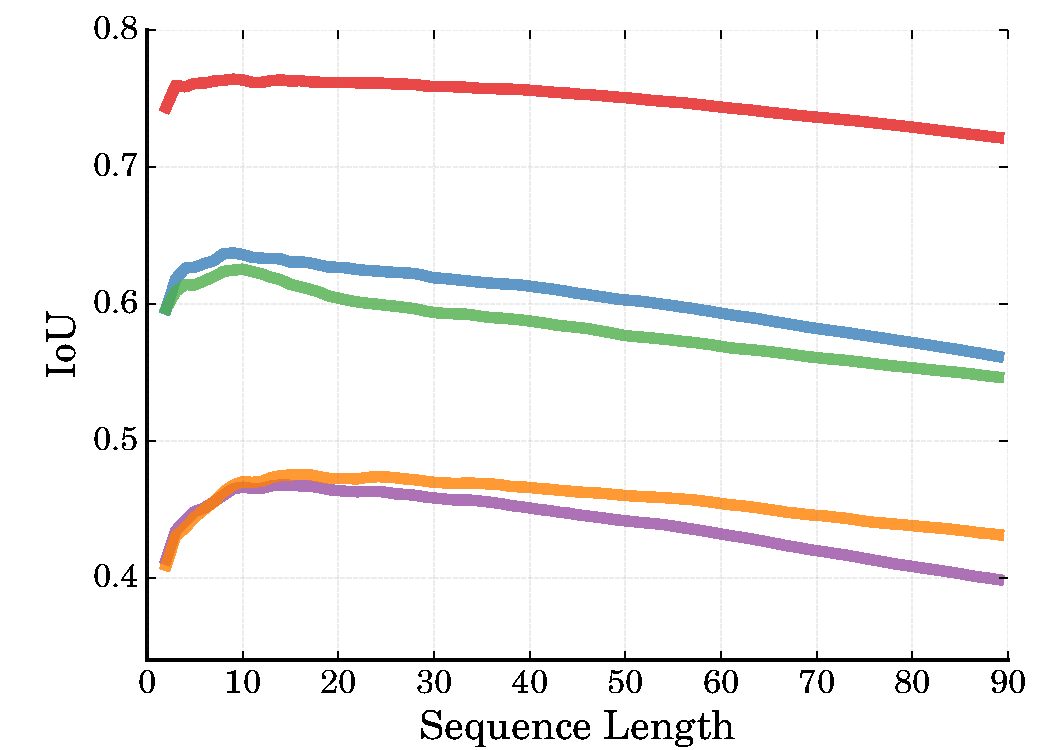
\includegraphics[width=\linewidth]{figures/MOHART/toy_iou_over_timesteps.pdf}
    \end{subfigure}
    \begin{subfigure}[c]{0.49\linewidth}
        \centering
        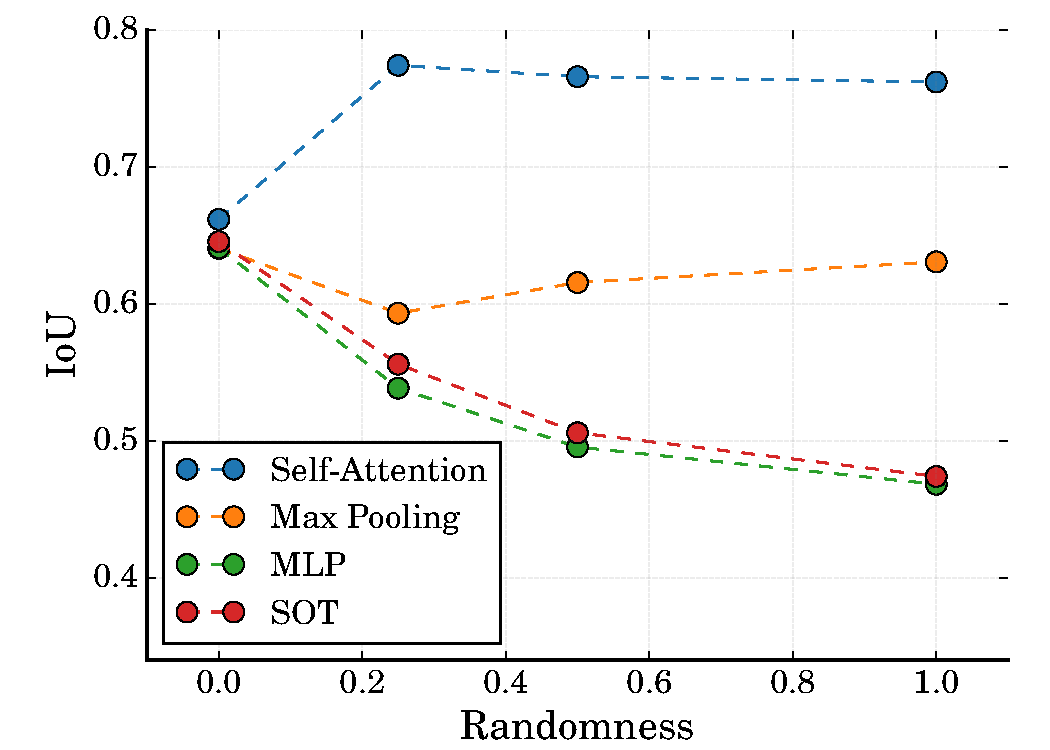
\includegraphics[width=\linewidth]{figures/MOHART/dial.pdf}
    \end{subfigure}
    \vspace{-2mm}
    \caption{
        Left: average IoU over sequence length for different implementations of relational reasoning on the toy domain shown in \cref{fig:toy2} ($\text{randomness} = 1.0$). Right: performance depending on how often agents are re-assigned identities randomly (sequence length 15). The higher the randomness, the less static the force field is and the more vital relational reasoning is. For $\text{randomness} = 0.0$, identities still have to be reassigned in some cases in order to prevent deadlocks, this leads to a performance loss for all models, which explains lower performance of self-attention for $\text{randomness} = 0.0$.
        \vspace{-4mm}
    }
    \label{fig:toy_quant}
\end{figure}

In the second experiment, we introduce randomness, rendering the scenario not solvable for a single object tracker as it requires knowledge about the state of the other objects and relational reasoning (see \cref{fig:toy2}). In each time step, we assign a colour-coded identity to the objects. Objects of the same identity repel each other, object of different identities attract each other (the objects can be thought of as electrons and protons). The qualitative results in \cref{fig:toy2} show that \textsc{mohart}, using self-attention for relational reasoning, is able to capture these interactions with high accuracy.
\Cref{fig:toy_quant} (left) shows a quantitative comparison of augmenting \textsc{hart} with different relational reasoning modules when identities are re-assigned in every timestep ($\text{randomness} = 1.0$). Exchanging information between trackers of different objects in the latent space with an MLP leads to slightly worse performance than the \textsc{HART} baseline, while simple max-pooling performs significantly better ($\Delta \text{IoU} \sim 17\%$). This can be explained through the permutation invariance of the problem: the list of latent representation of the different objects has no meaningful order and the output of the model should therefore be invariant to the ordering of the objects. The MLP is in itself not permutation invariant and therefore prone to overfit to the (meaningless) order of the objects in the training data. Max-pooling, however, is permutation invariant and can in theory, despite its simplicity, be used to approximate any permutation invariant function given a sufficiently large latent space \citep{Wagstaff2019}. Max-pooling is often used to exchange information between different tracklets, e.g., in the trajectory prediction domain \citep{Alahi2016social,Gupta2019social}. However, self-attention, allowing for learned querying and encoding of information, solves the relational reasoning task significantly more accurately. In \cref{fig:toy_quant} (right), the frequency with which object identities are reassigned randomly is varied. The results show that, in a deterministic environment, tracking does not necessarily profit from relational reasoning - even in the presence of long-range interactions. The less random, the more static the force field is and a static force field can be inferred from a small number of observations (see \cref{fig:toy1}). This does not mean that all stochastic environments profit from relational reasoning. What these experiments indicate is that tracking can not be expected to profit from relational reasoning by default in any environment, but instead in environments which feature (potentially non-deterministic) dynamics and predictable interactions.